\subsection{\mbox{RX~J1347.5-1145} as observed by {\it NIKA}}
\label{sec:result_map}
Figure~\ref{fig:rxj} presents the \mbox{RX~J1347.5-1145} tSZ map obtained with the {\it NIKA} prototype. The radio source is subtracted in the right panel but not in the left panel. The associated difference map of separated equivalent subsamples (Jack-Knife), which is normalized by a factor of 2 to preserve the statistical properties of the noise in the tSZ map, is given in the left panel of Fig.~\ref{fig:rxj_jk}. We also present on the middle panel of Figure~\ref{fig:rxj_jk} the histogram of the pixel values. The outside contour of the maps shown is defined by the limit where the statistical noise level, which increases toward the edges of the full map, equals twice the minimum noise level of the inner region. The bottle-like shape of the cut-off is due to the scan strategy detailed in Sect.~\ref{sec:obs_condition}. \\

The inhomogeneity of the noise can be seen directly on the half difference map in Fig.~\ref{fig:rxj_jk}. This is even more obvious on the histogram plot that provides the noise distribution in two different regions of the half difference map and on the standard deviation map. We observe that the standard deviation on the two regions is significantly different,  $<\sigma> = 0.99$~mJy/beam on the east side and $<\sigma> = 1.42$~mJy/beam on the west side. From the half difference map, we estimate the overall root mean square of the noise in the cluster map to $<\sigma> = 1.11$~mJy/beam. This is obtained by fitting the histogram of the pixel value with a Gaussian distribution. The contours overplotted on the tSZ maps of Fig.~\ref{fig:rxj} correspond to 3, -3, -6, and -9~mJy/beam with the noise level being $1 \sigma \cong 1$~mJy/beam at the cluster location. The beam is shown on the bottom left corner of the map, accounting for both the 18.5~arcsec instrumental beam and the extra 10~arcsec Gaussian smoothing of the map ({\it i.e.}, 21~arcsec). In terms of the Compton parameter, the sensitivity of the {\it NIKA} prototype camera during the campaign of November 2012 is $\sim 10^{-4} \sqrt{\mathrm{h}}$ for one beam and 1$\sigma$.
	
The maps in Fig.~\ref{fig:rxj} clearly show the tSZ decrement that reaches up to $\simeq 10 \ \sigma$. The signal is extended, and its maximum does not coincide with the \mbox{X-ray} center, (R.A,~Dec)~=~(13h~47m~30.59s,~-11$^{\mathrm{o}}$~45'~10.1"). It corresponds to the shock location, even for the radio point source subtracted map, which agrees with other single-dish observations.  As mentioned in Sect.~\ref{sec:previous_obs}, these results do not agree with those from {\it CARMA} interferometric \mbox{RX~J1347.5-1145}  observations \citep{plagge_2012}. The tSZ maximum corresponds to $\simeq 10^{-3}$ in units of Compton parameter $y$, as expected for this cluster according to \cite{pointecouteau_1999}. The consistency of the NIKA  \mbox{RX~J1347.5-1145} map with previous observations is further discussed in Sect.~\ref{sec:comparison}.
	 
	\begin{figure*}
	\centering
	\includegraphics[width=0.45\textwidth]{Figure/RXJ1347-1145_map_2mm}
	\hspace*{0.5cm}
	\includegraphics[width=0.45\textwidth]{Figure/RXJ1347-1145_map_2mm_pointsource_sub}
	\caption{{\it NIKA} map of \mbox{RX~J1347.5-1145} at 140~GHz. Left: Original {\it NIKA} map with the radio source not subtracted. Right: Same map with the radio source subtracted. The maps are given in~mJy/beam. They are clipped up to a root mean square noise level that is twice the minimum of the map as detailed in the text. The contours are at 3, -3, -6 and -9~mJy/beam with $1 \sigma \cong 1$~mJy/beam at the cluster location. The minimum value of the maps corresponds to $y \simeq 10^{-3}$. The \mbox{X-ray} center location is represented by a white cross. The radio source location also corresponds to the white cross within 3~arcsec. The locations of the two infrared galaxies are given as red stars.}
        \label{fig:rxj}
	\end{figure*}
	
	\begin{figure*}
	\centering
	\includegraphics[width=0.31\textwidth]{Figure/JK_smallFOV}
	\hspace*{0.3cm}
	\includegraphics[width=0.31\textwidth]{Figure/histo_jk_smallFOV2}
	\hspace*{0.3cm}
	\includegraphics[width=0.31\textwidth]{Figure/RXJ1347-1145_map_rms}
	\caption{\mbox{RX~J1347.5-1145} observations. Left: Half-difference map of two equivalent subsamples mimicking the noise properties of the tSZ map. The pixels are 2$\times$2~arcsec, and the map has been smoothed with a 10~arcsec Gaussian filter, which is similar to the tSZ map of Fig.~\ref{fig:rxj}. The noise level is not homogeneous, which is lower on the left hand side, due to the differences of acquisition time. Middle: Noise distribution obtained from the half difference map. Since the noise is not homogeneous, we provide the distribution for both the eastern (left, green) and western (right, red) parts of the map. A Gaussian fit of the histograms gives the mean value of the standard deviation of the noise to be $<\sigma> = 0.99$~mJy/beam on the east side and $<\sigma> = 1.42$~mJy/beam on the west side. The minimum noise level reaches 0.8~mJy/beam. The contours of the noise map (left) correspond to the overall mean noise (i.e.  $\pm 1.11$ mJy/beam). Right: Standard deviation map estimated from difference maps. White regions have not been observed. Gray regions are those for which the standard deviation is higher than 6~mJy/beam.}
        \label{fig:rxj_jk}
	\end{figure*}
	
\subsection{\mbox{RX~J1347.5-1145} profile}
\label{sec:profile}
Figure~\ref{fig:profiles} gives the flux profile as a function of the angular distance that is extracted from the tSZ map in Fig.~\ref{fig:rxj}. In the case of \mbox{RX~J1347.5-1145}, the tSZ barycenter and the \mbox{X-ray} center do not coincide due to the ongoing merger. We compare the profile computed from the \mbox{X-ray} center, (R.A,~Dec)~=~(13h~47m~30.59s,~-11$^{\mathrm{o}}$~45'~10.1"), to the tSZ peak that is taken to be at the coordinates (R.A,~Dec)~=~(13h~47m~31s,~-11$^{\mathrm{o}}$~45'~30") from the maximum decrement of the {\it NIKA} map. The error bars have been computed from simulated noise maps with statistical properties estimated using the half-difference map presented on the left panel of Fig.~\ref{fig:rxj_jk}.

The right panel in Fig.~\ref{fig:profiles} compares the profile of \mbox{RX~J1347.5-1145} from the \mbox{X-ray} center in three different areas: the northwest, the northeast, and the south. It shows the increase in thermal pressure in the southern region, where the subclump (merging) is observed in \mbox{X-ray} and tSZ (Sect.~\ref{sec:previous_obs}). This is due to the compression of the hot gas within the merging process, which increases the temperature and thus the pressure (deepening the tSZ decrement at 140~GHz). We note that the southern extension coincides with the presence of a radio mini-halo \citep[see the work by][]{gitti_2007_bis}, which implies the presence of non-thermal electrons that could underline a non-thermal contribution to the total pressure (not seen in the tSZ signal). We also note that the radio source has been subtracted before the calculation of the profiles.
	\begin{figure*}
	\centering
	\includegraphics[width=0.45\textwidth]{Figure/profile_SZvsX}
	\hspace*{0.5cm}
	\includegraphics[width=0.45\textwidth]{Figure/profile_pie}
	\caption{Radial flux profiles of \mbox{RX~J1347.5-1145}. Left: Comparison of the radial profile computed from the \mbox{X-ray} (red dots) and tSZ (green diamonds) centers. Right: Comparison of the radial flux profile in three different regions from the \mbox{X-ray} center. The map is cut from the \mbox{X-ray} center in three equal slices: one cut is vertical coming from the north to the center, and the two others are diagonal from the southeast and the southwest to the center, respectively. The red diamonds and yellow dots profiles correspond to the northwest and northeast part of the map, respectively, where the cluster is expected to be rather relaxed. The green triangle profile corresponds to the southern part of the map, where the merging occurred.}
        \label{fig:profiles}
	\end{figure*}

\subsection{Modeling of the cluster pressure profile}
\label{sec:mcmc}
The object \mbox{RX~J1347.5-1145} has been intensively studied in \mbox{X-rays}, which have revealed a fairly regular cluster at a large scale down to the center in the north direction with a low central entropy~\citep{Cavagnolo2009}. The contrast with the southern part, which exhibits a tSZ and \mbox{X-ray} extension, suggests that \mbox{RX~J1347.5-1145} was a spherical, relaxed cool-core cluster that is undergoing the merging of a subcluster on its southern part. We, therefore, aim at quantifying the tSZ South East extension detected with the {\it NIKA} prototype by modeling and subtracting the signal coming from the relaxed region, which is located on the northern-west side of the \mbox{X-ray} center. We model the tSZ signal by considering a gNFW profile (Eq.~\ref{eq:gNFW}), which is centered at the \mbox{X-ray} position of the system, whose inner, outer, and intermediate slopes ($\gamma$, $\beta$, $\alpha$) have been set equal to the cool-core best-fitting values of \cite{arnaud_2010} ($\gamma_\mathrm{cc} = 0.7736$, $\beta_\mathrm{cc} = 5.4905$, $\alpha_\mathrm{cc} = 1.2223$). The best-fitting values of $P_{0}$ and $\theta_s$ are obtained using a Markov Chain Monte Carlo (MCMC) approach. The sequence of random samples, known as the chain, has been built by implementing the Metropolis-Hasting algorithm \citep{Greenbert95}, which means that the parameter space is explored with a trial step drawn from a symmetric probability distribution. Convergence of the chains is checked by including the test proposed by \cite{GelmanRubin1992}.

	\begin{figure}	
	\centering
	\includegraphics[width=\columnwidth]{Figure/lik_mask80_rxj_comp.pdf}	
	\caption{Posterior likelihood of the MCMC pressure profile fit in the plane $P_0$ -- $\theta_s$. From dark to light blue, the colors correspond to 68\%, 95\%, and 99\% confidence levels. The top and right curves show the normalized Gaussian best fit of the marginalized likelihood of $P_0$ and $\theta_s$, respectively.}
        \label{fig:likelihood}
	\end{figure}

The parameters $P_{0}$ and $\theta_s$ have been constrained by masking the southeast extension. The mask has been defined as a half ring on the southern part of the cluster, centered on the \mbox{X-ray} peak with inner and outer radii set to 10 and 80~arcsec, respectively. By masking the hottest region of the system, the constraints obtained on the best fit parameters are mainly driven by the cool-core like component, where the cluster temperature remains below 10 keV. Consequently, the flux relativistic correction \citep{itoh_1998, nozawa1998, nozawa2006} is estimated to be $\lesssim$ 7\% at 140 GHz and needs to be propagated to the following results. The best fit parameters obtained are
    	\begin{eqnarray}
	P_{0} & = & 0.129 \pm 0.018 \ (\mathrm{stat.}) \ \pm^{0.035}_{0.025} \ (\mathrm{syst.}) \ \mathrm{keV/cm}^3 \  {\rm and}\nonumber \\
	\theta_s & = &  1.90 \pm 0.16 \ (\mathrm{stat.}) \ \pm^{0.38}_{0.00} \ (\mathrm{syst.}) \ \mathrm{arcmin}.  
	\label{eq:best_fit_nika}
	\end{eqnarray}
The corresponding posterior likelihood is given in Fig.~\ref{fig:likelihood} and accounts for statistical uncertainties only. The systematic uncertainties have been computed by using the calibration uncertainty and considering the bias filtering effect of the analysis that is estimated from the simulations described in Sect.~\ref{sec:sz_simu}. The pressure profile normalization parameter, $P_{0}$, is symmetrically affected by the calibration uncertainty, while the negative bias (lowering the true value) has been estimated to less than 20\%. The parameter $\theta_s$ is only affected by the bias, which is estimated to less than 20\% and lowers its true value. 

Figure~\ref{fig:residual} compares the {\it NIKA} prototype point source subtracted map with the best fit model obtained for the relaxed component, and the residual. The model represents the northern part of the tSZ map well, but the southern side cannot be explained without including an overpressure component, which is known to be due to the merging of a subcluster (see Sect.~\ref{sec:previous_obs}).

The best fit model and the residual tSZ map, as given in Fig.~\ref{fig:residual}, have been used to quantify the distribution of the signal within the region, where the intracluster gas is more relaxed toward hydrostatic equilibrium, and the region, where it is expected to be shock heated. For this purpose, we compute the integrated Compton parameter, as defined as 
	\begin{equation}
	Y_{\theta_{\mathrm{max}}} =  \int_{\Omega(\theta_{\mathrm{max}})} y \ d\Omega,
	\label{eq:y_integ}
 	\end{equation}
	over the solid angle $\Omega$ up to the radius $\theta_{\mathrm{max}}$ from the \mbox{X-ray} center. This is separately done on the map and the residual (as seen in Fig.~\ref{fig:residual}). Given the size of the NIKA map, we integrate up to $\theta_{\mathrm{max}}$~=~2~arcmin. The total integrated Compton parameter within this radius is $Y^{\mathrm{total}}_{\theta_{\mathrm{max}}} =  (1.73 \pm 0.45) \times 10^{-3}$~arcmin$^2$. After removing the best fit cool-core model and integrating the residual in the same region, we obtain $Y^{\mathrm{shock}}_{\theta_{\mathrm{max}}} = (0.52 \pm 0.18) \times 10^{-3}$~arcmin$^2$. The errors on the integrated fluxes account for the statistical noise only. Systematic uncertainties are estimated to be of the order of 19\%. Thus, the shock contribution is estimated to be ($30 \pm 13 \pm 6$)~\% of the total tSZ flux at these small cluster-centric distances. Considering the {\it Planck} $Y_{5R_{500}}$ measurements \citep{Planck_fit}, the shock contribution corresponds to about 24 \% of the total tSZ flux. Previous observations by \cite{mason_2010} and \cite{plagge_2012} are consistent with a lower relative contribution of the shock of 9 to 10 \%. A direct comparison of these results with ours is difficult because of the very different methodologies used. In particular, the angular scales probed by the different instruments are not the same. Furthermore, \cite{mason_2010} and \cite{plagge_2012} have used external data to compute the overall tSZ flux, while we use {\it NIKA} data only in this paper.

	\begin{figure*}	
	\centering	
	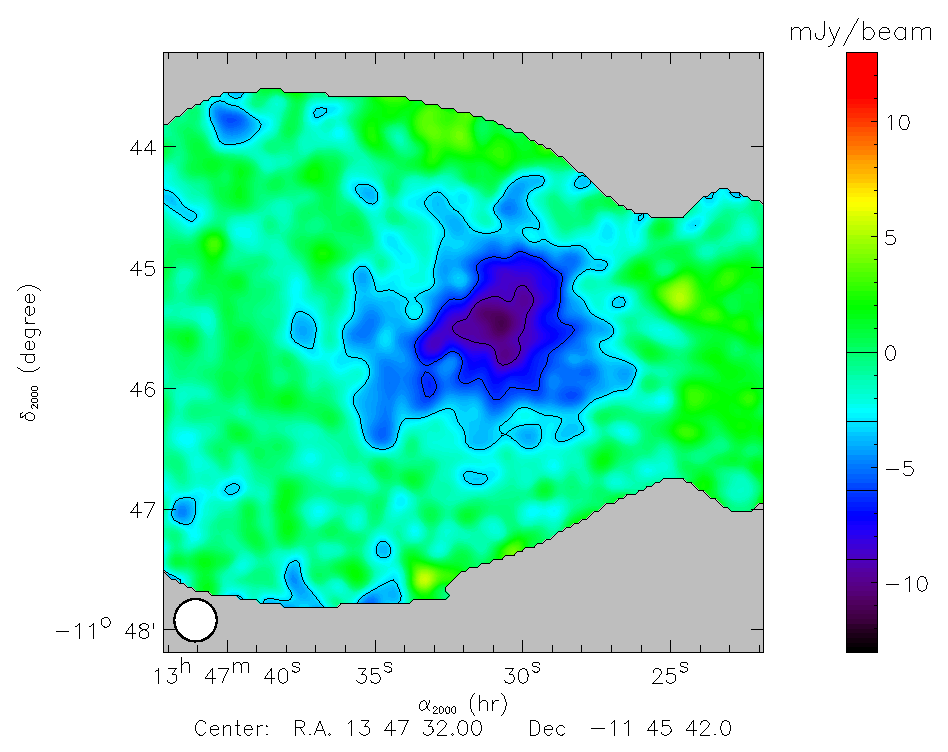
\includegraphics[width=0.3\textwidth]{Figure/RXJ1347-1145_PS_subtracted_map_2mm}
	\hspace*{0.3cm}
	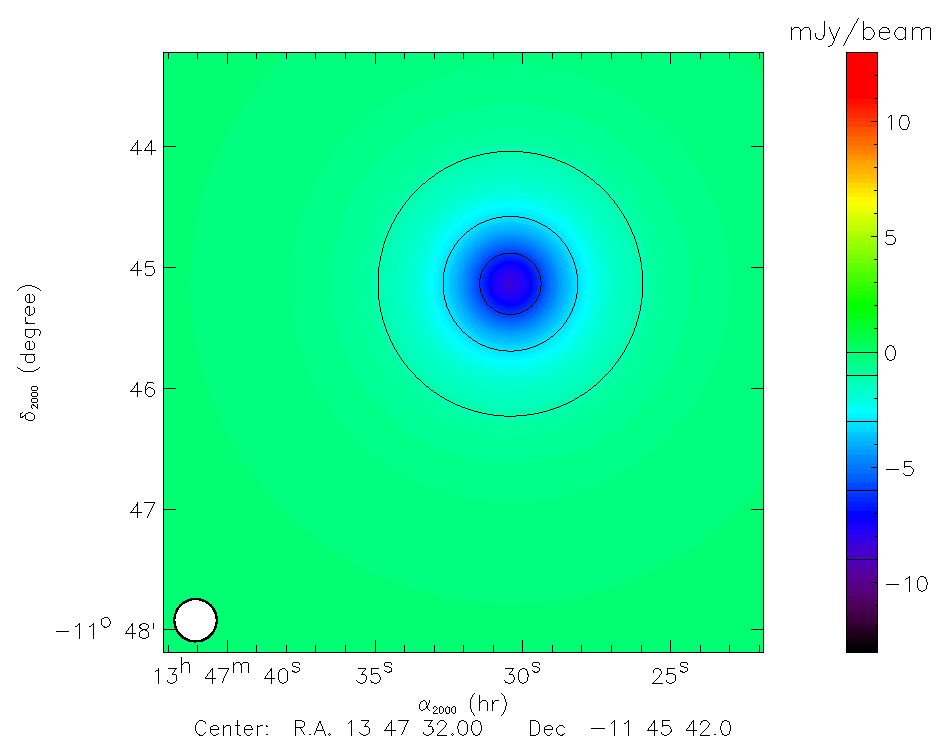
\includegraphics[width=0.3\textwidth]{Figure/model}
	\hspace*{0.3cm}
	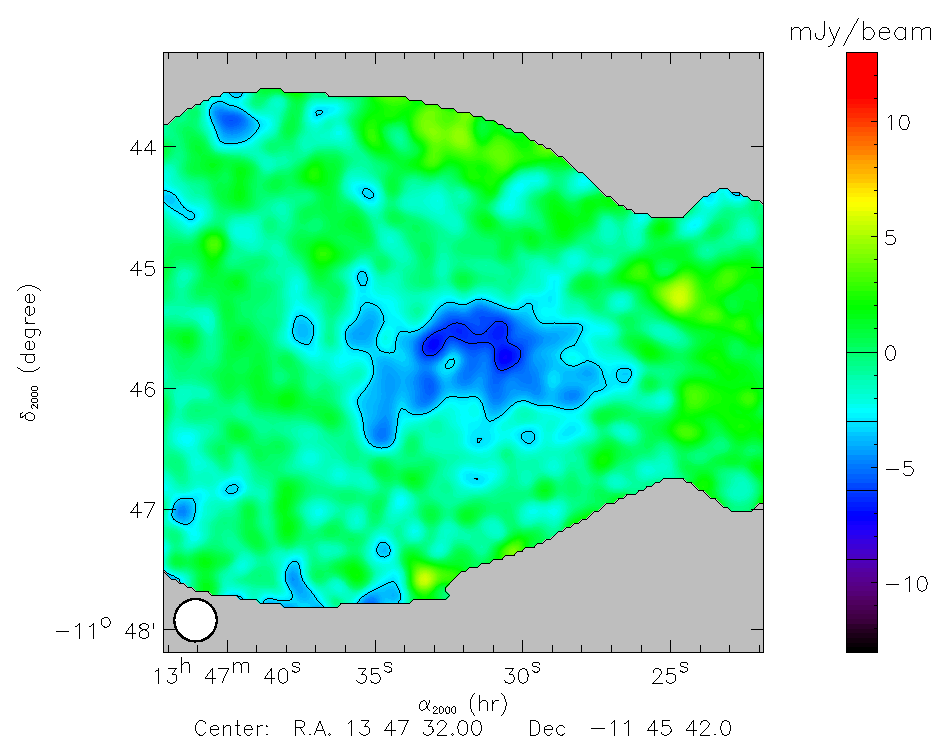
\includegraphics[width=0.3\textwidth]{Figure/residu}
	\caption{Comparison between the original point source subtracted \mbox{RX~J1347.5-1145} tSZ map (left panel) and the best fit model map excluding the shock area (middle panel). The residuals are given on the right panel map. The model accounts for the cluster emission well, except in the southern shocked area, as expected.}
        \label{fig:residual}
	\end{figure*}
	